\documentclass[conference, twocolumn]{IEEEtran}

\usepackage[utf8]{inputenc}
\usepackage[T1]{fontenc}
\usepackage{amsmath, amssymb}
\usepackage{graphicx}
\usepackage{listings}
\usepackage{xcolor}
\usepackage{hyperref}
\usepackage{booktabs}
\usepackage{float}

% Code listing style
\lstset{
  language=Python,
  basicstyle=\ttfamily\scriptsize,
  keywordstyle=\color{blue}\bfseries,
  commentstyle=\color{gray}\itshape,
  stringstyle=\color{red},
  breaklines=true,
  frame=single,
  numbers=left,
  numberstyle=\tiny\color{gray},
  columns=fullflexible,
  keepspaces=true
}

\title{Aerial Robotics Kharagpur Documentation\\Task 2.3 -- Medial Axis Detection of Moving Surgical Tools}

\author{Parv Chopra *}

\begin{document}

\maketitle

% ============================================================================
%  ABSTRACT
% ============================================================================
\begin{abstract}
This report presents a computer vision pipeline for detecting the medial axis (centreline) of moving surgical tools in video. The final pipeline consists of per-pixel median background subtraction, morphological closing, Sobel-based edge detection, and a fully custom Hough Line Transform implemented from scratch. Edge pairs are selected using a geometrically robust criterion (intersection filtering combined with angular-difference ranking) and the medial axis is computed as the angular bisector of the two dominant edge lines rather than a simple parameter average. The output is an annotated video with green edges and a red medial axis overlaid on each frame. This pipeline finds application in surgical robotics and computer-assisted intervention, where real-time tool-axis estimation is essential for autonomous or semi-autonomous operation.
\end{abstract}

% ============================================================================
%  I. INTRODUCTION
% ============================================================================
\section{Introduction}

The objective of Task~2.3 is to detect the medial axis (centreline) of a moving surgical tool in video footage. The medial axis is the line equidistant from both edges of the tool; it represents the tool's orientation and position.

Key constraints of the task:
\begin{itemize}
    \item \textbf{No built-in Hough Transform}: \texttt{cv2.HoughLines} and \texttt{cv2.HoughLinesP} are not allowed. The Hough Line Transform must be implemented from scratch.
    \item The pipeline must work on video (frame-by-frame processing).
    \item Output: overlay of detected edges (green) and medial axis (red) on each video frame.
\end{itemize}

The pipeline processes three videos and produces annotated output videos. Several approaches were explored iteratively, refining the background subtraction, edge-pair selection, and medial-axis computation at each stage until a robust final pipeline was reached.

% ============================================================================
%  II. PROBLEM STATEMENT
% ============================================================================
\section{Problem Statement}

Given video footage of a moving surgical tool:
\begin{enumerate}
    \item \textbf{Segment} the tool from the background.
    \item \textbf{Detect} the edges of the tool.
    \item \textbf{Find} the dominant edge lines using a custom Hough Transform.
    \item \textbf{Compute} the medial axis as the midline between opposite edges.
    \item \textbf{Overlay} edges and medial axis on each frame and produce output video.
\end{enumerate}

The primary constraint is that the Hough Line Transform must be implemented from scratch; no OpenCV Hough functions are permitted.

Figure~\ref{fig:pipeline_stages} shows four sample frames (from different videos) at each stage of the pipeline.

\begin{figure*}[t]
\centering
\begin{tabular}{cccc}
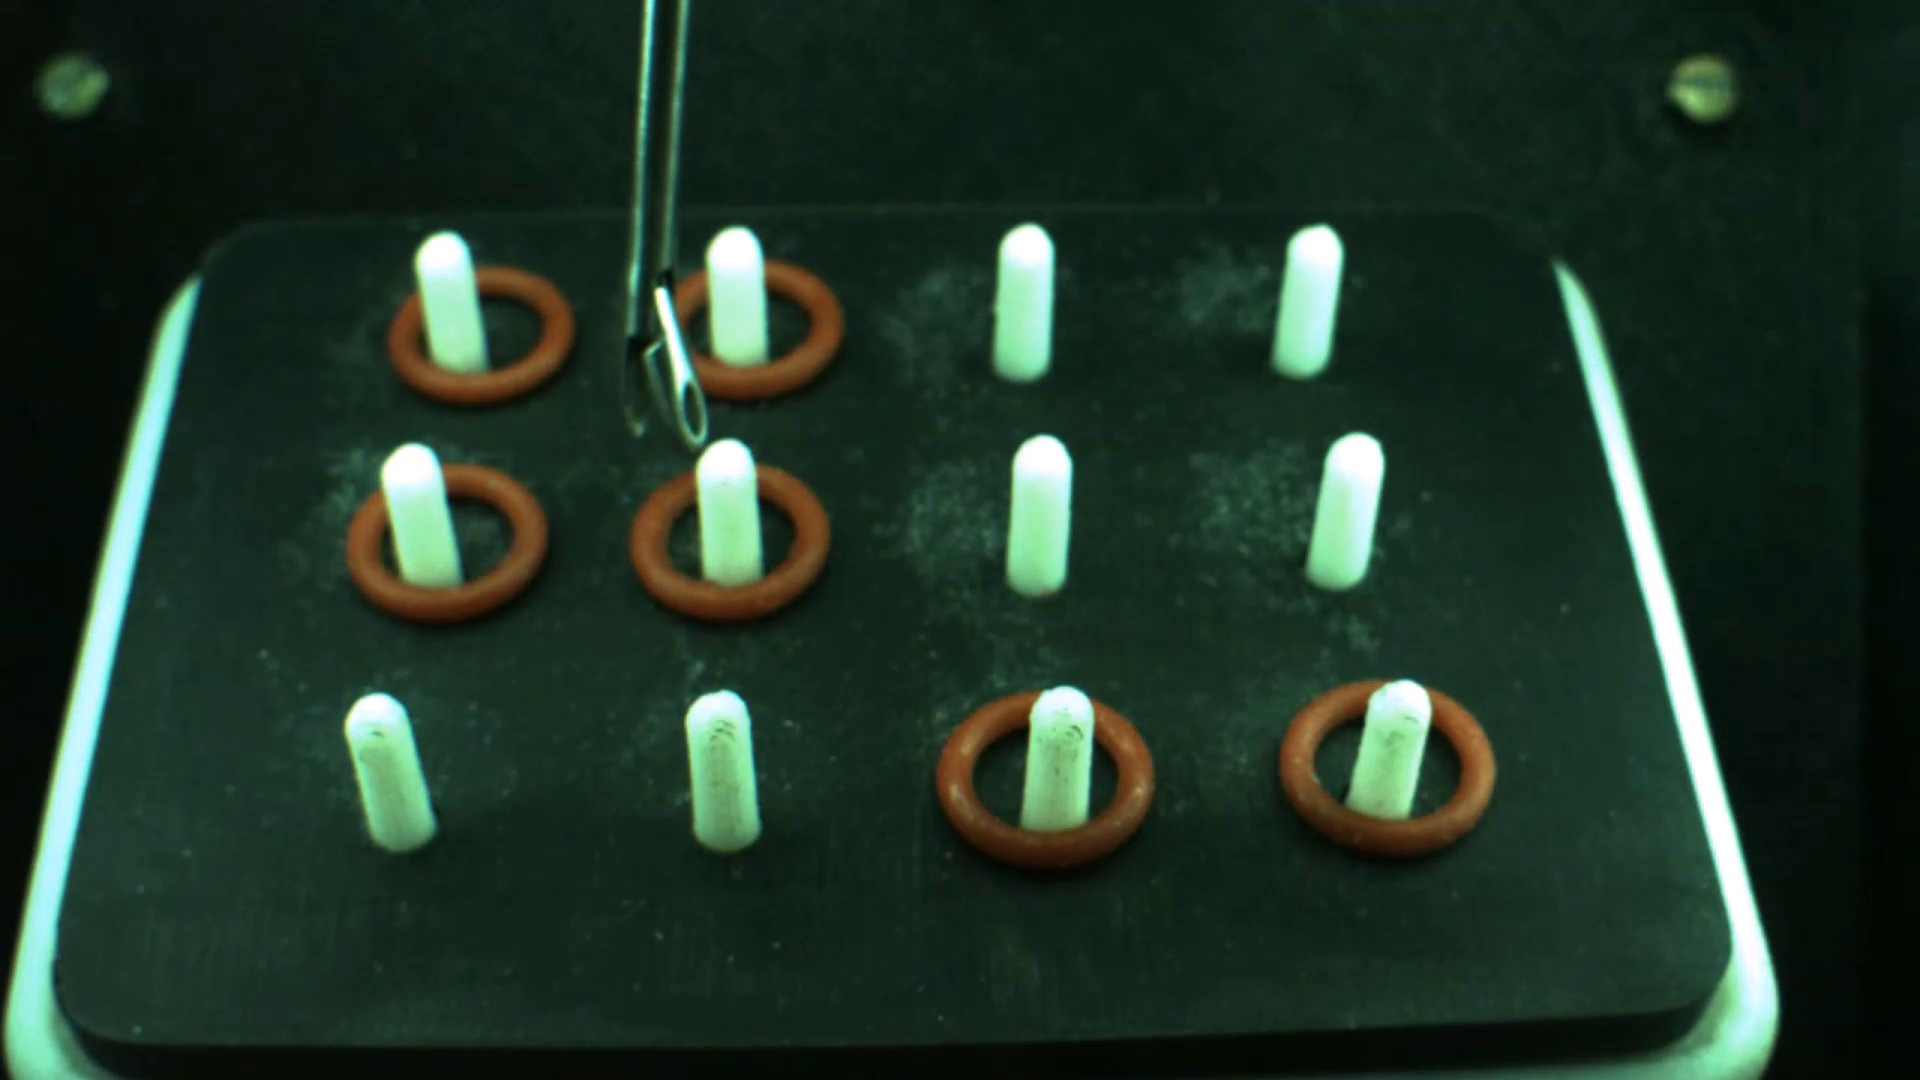
\includegraphics[width=0.23\textwidth]{output/frames/sample1_orig.jpg} &

\includegraphics[width=0.23\textwidth]{output/frames/sample1_fg.jpg} &

\includegraphics[width=0.23\textwidth]{output/frames/sample1_clean.jpg} &
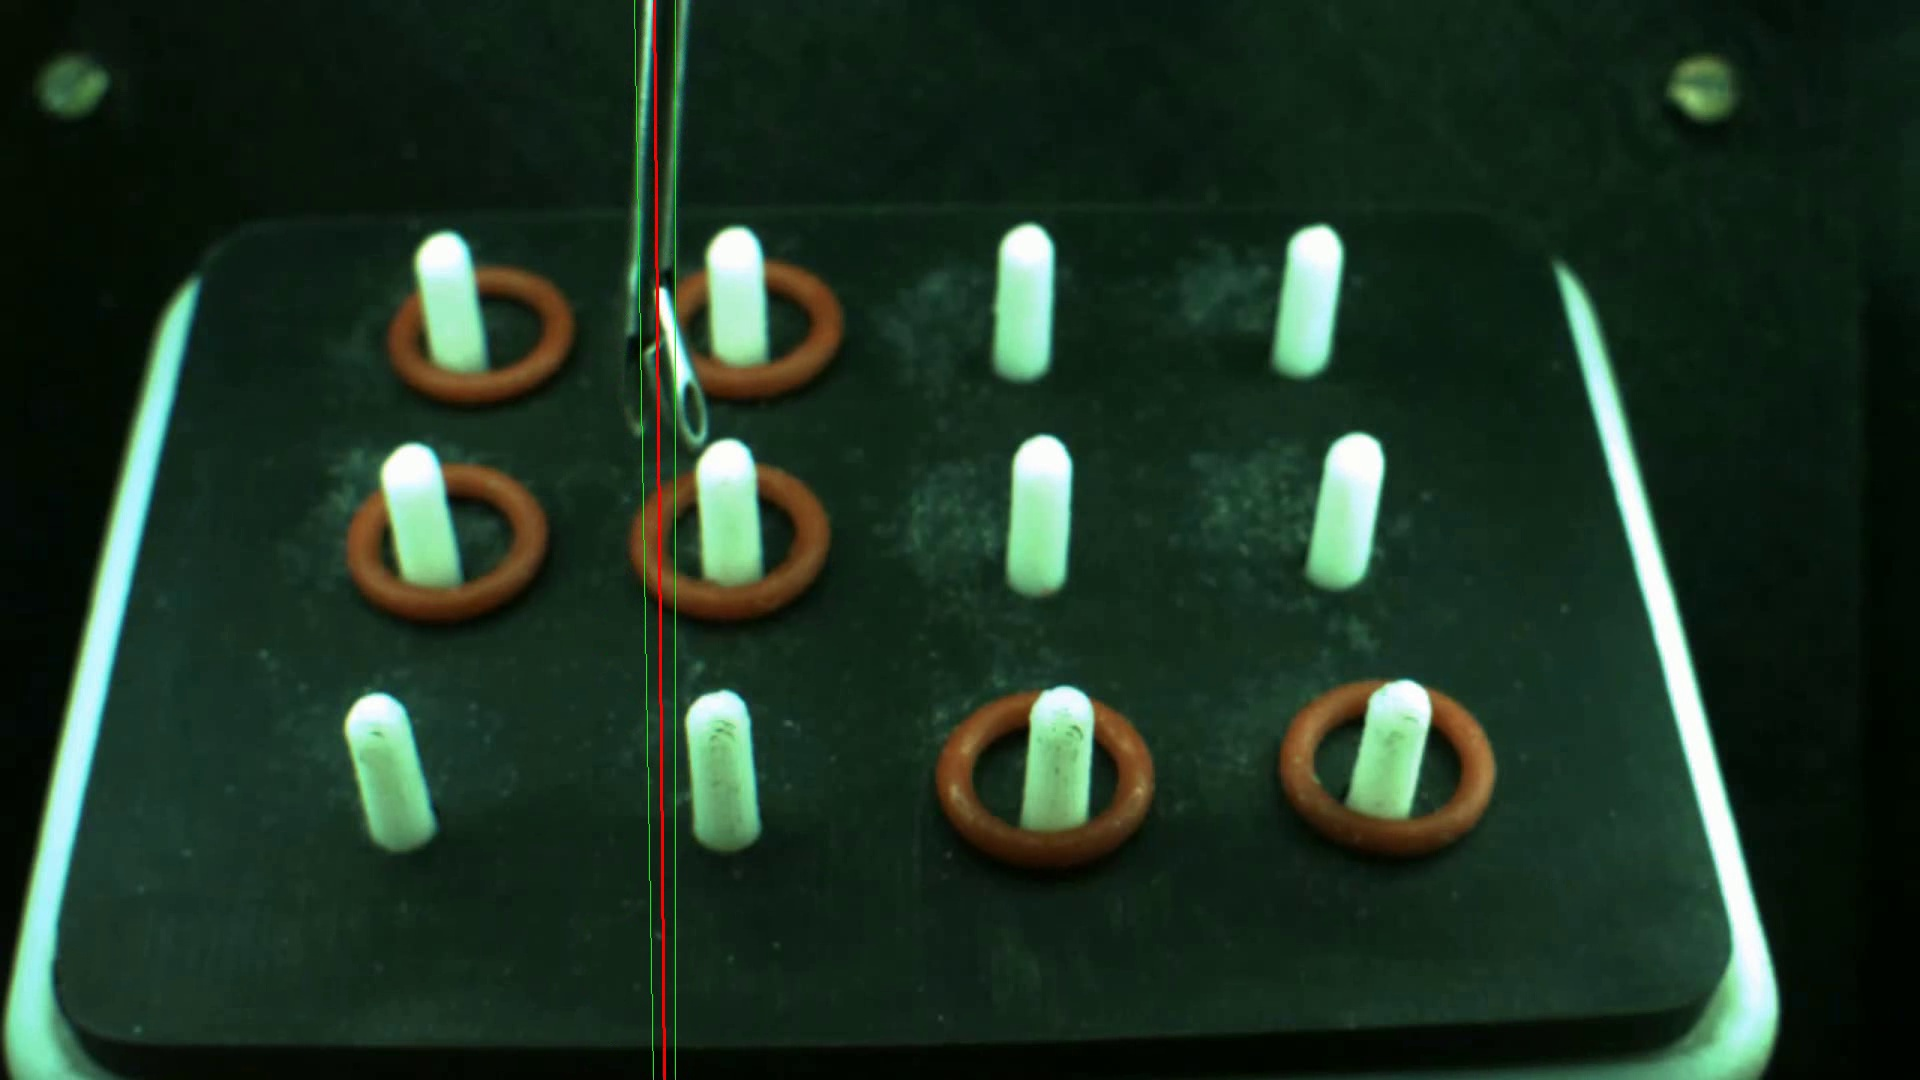
\includegraphics[width=0.23\textwidth]{output/frames/sample1_overlay.jpg} \\
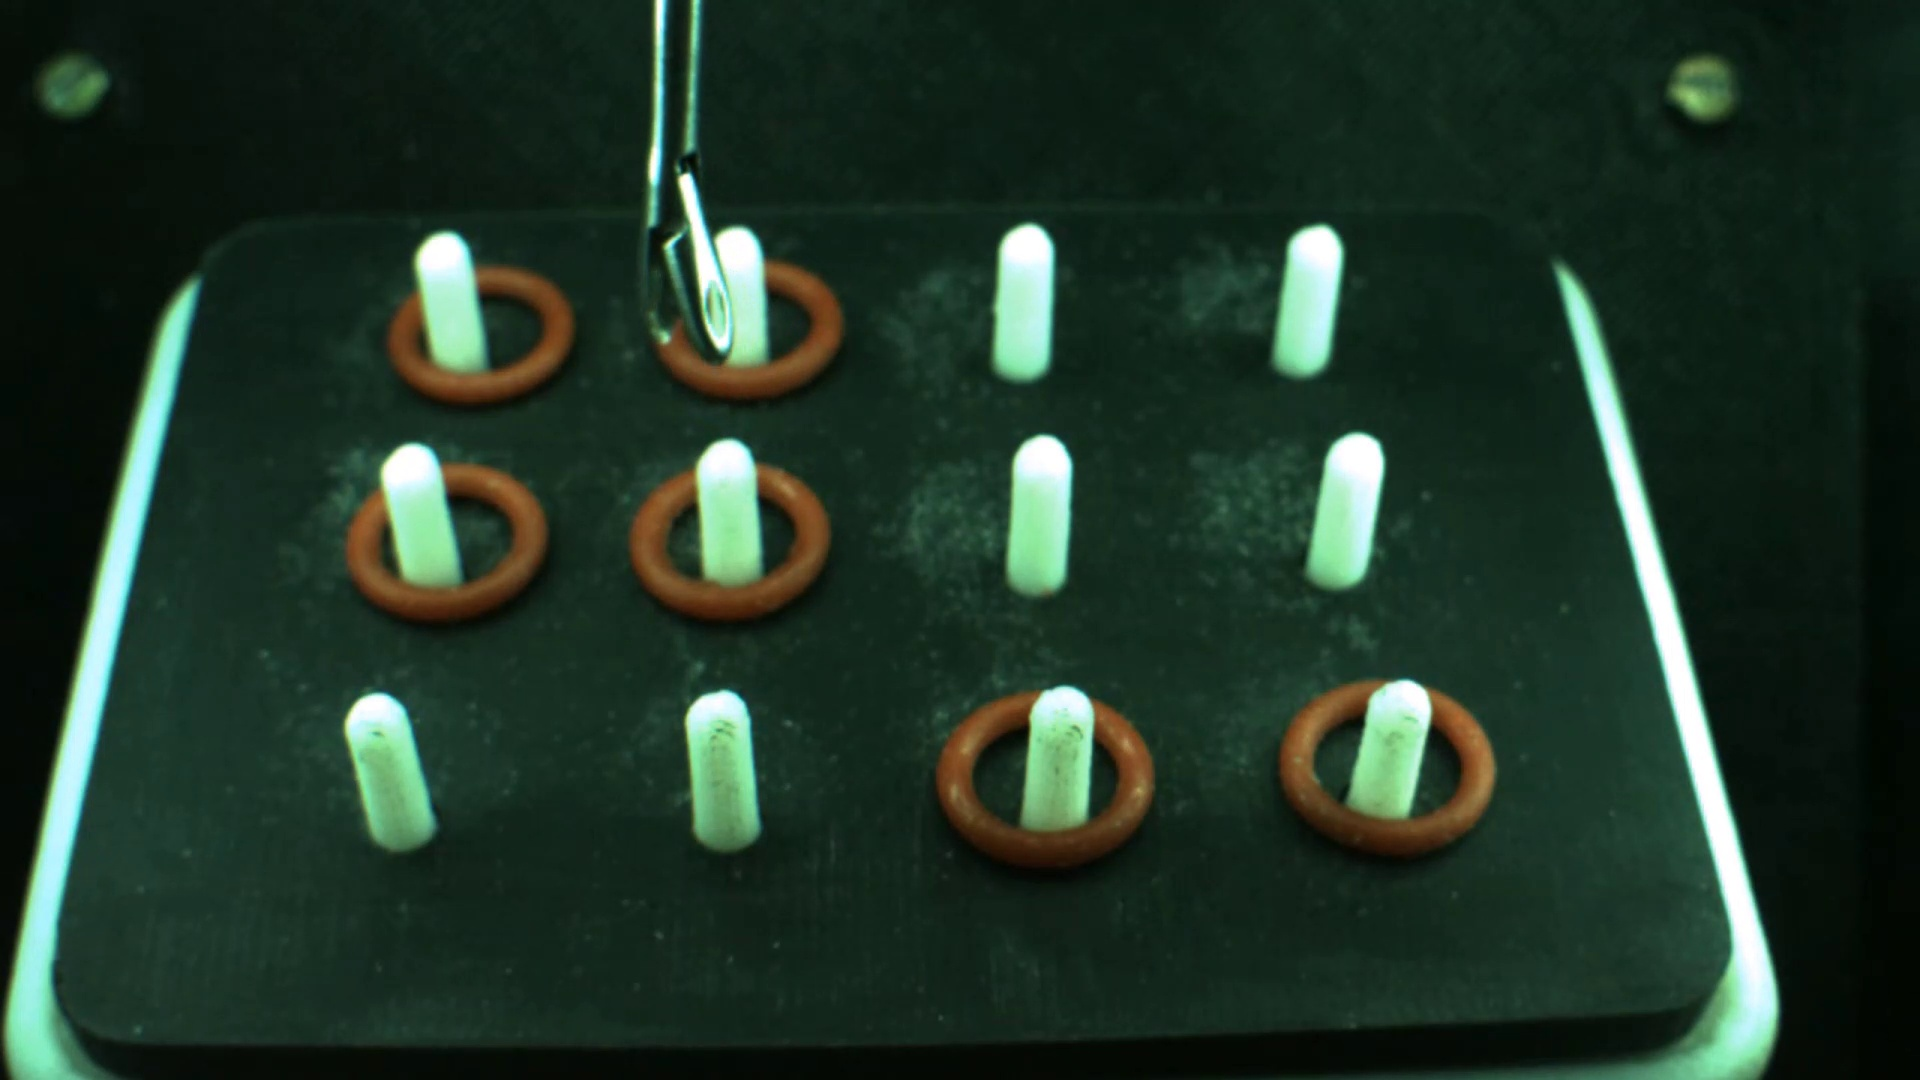
\includegraphics[width=0.23\textwidth]{output/frames/sample2_orig.jpg} &

\includegraphics[width=0.23\textwidth]{output/frames/sample2_fg.jpg} &

\includegraphics[width=0.23\textwidth]{output/frames/sample2_clean.jpg} &
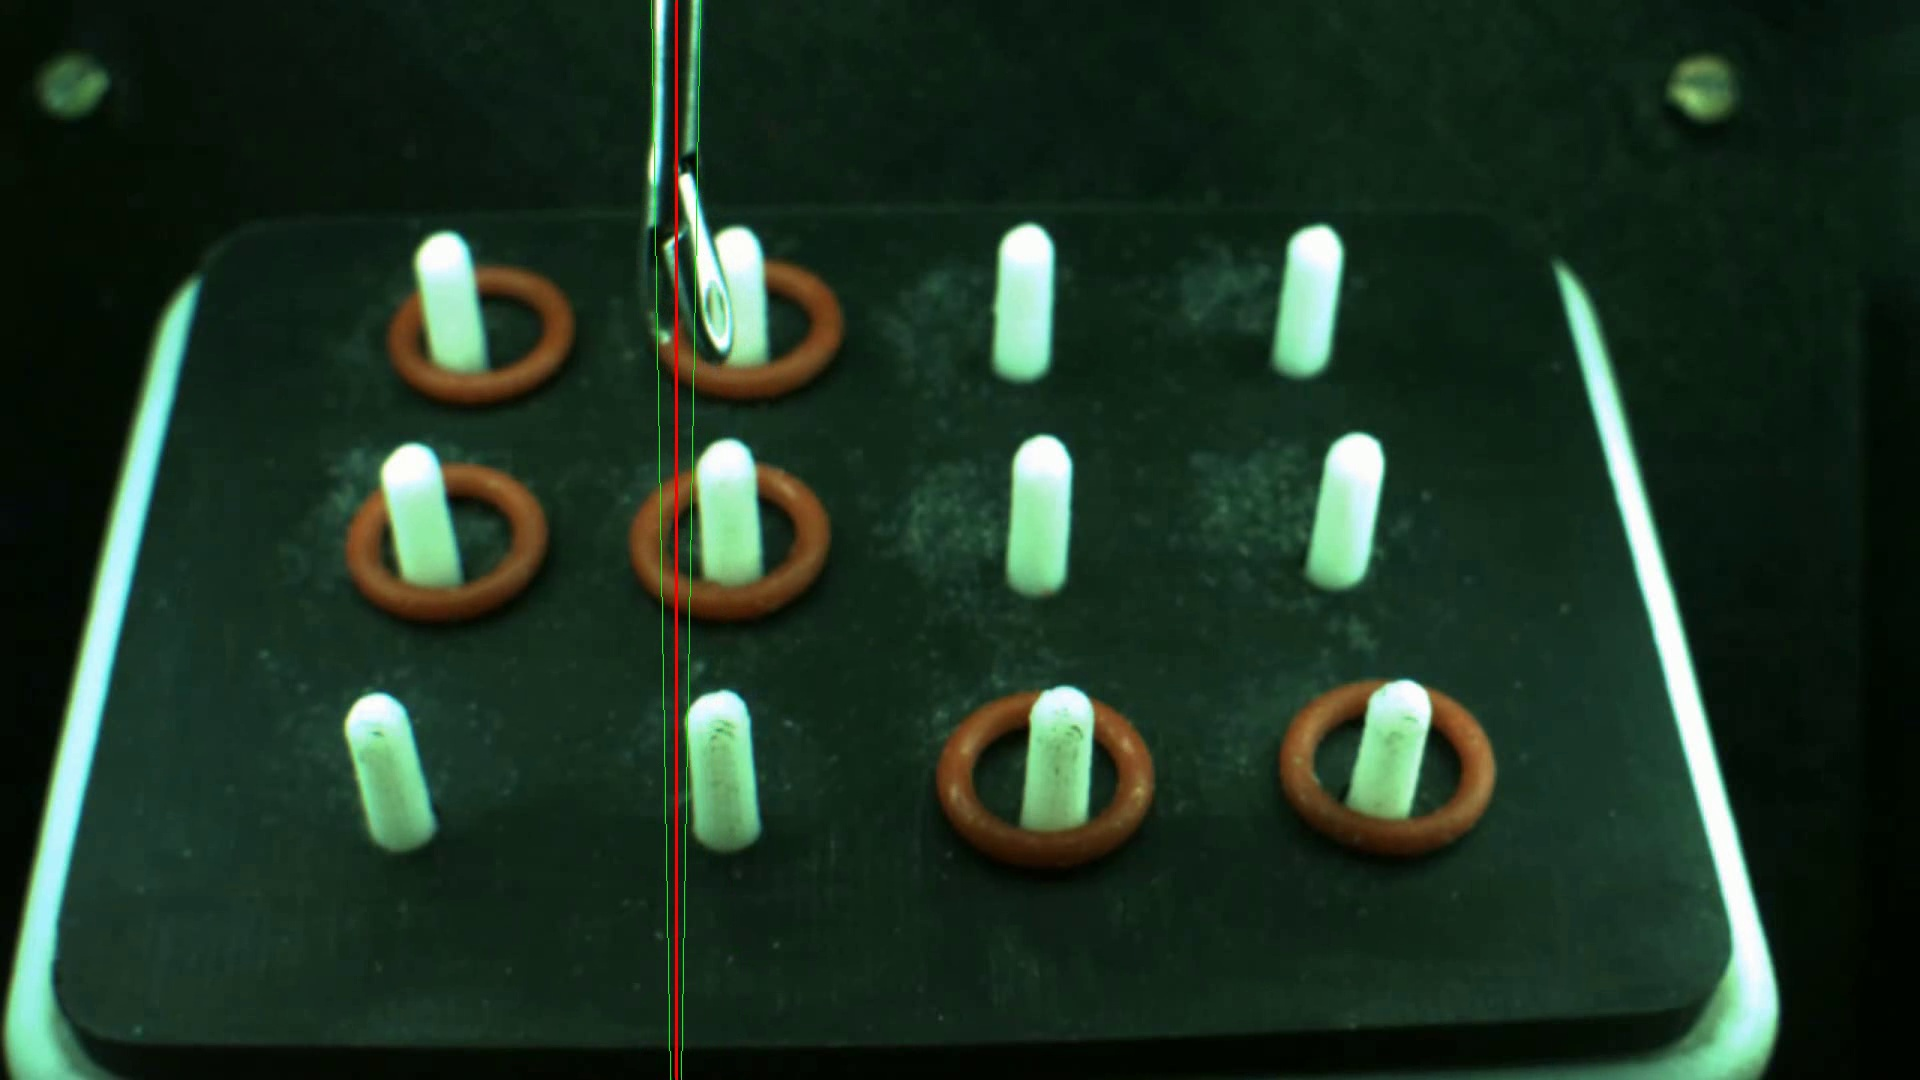
\includegraphics[width=0.23\textwidth]{output/frames/sample2_overlay.jpg} \\
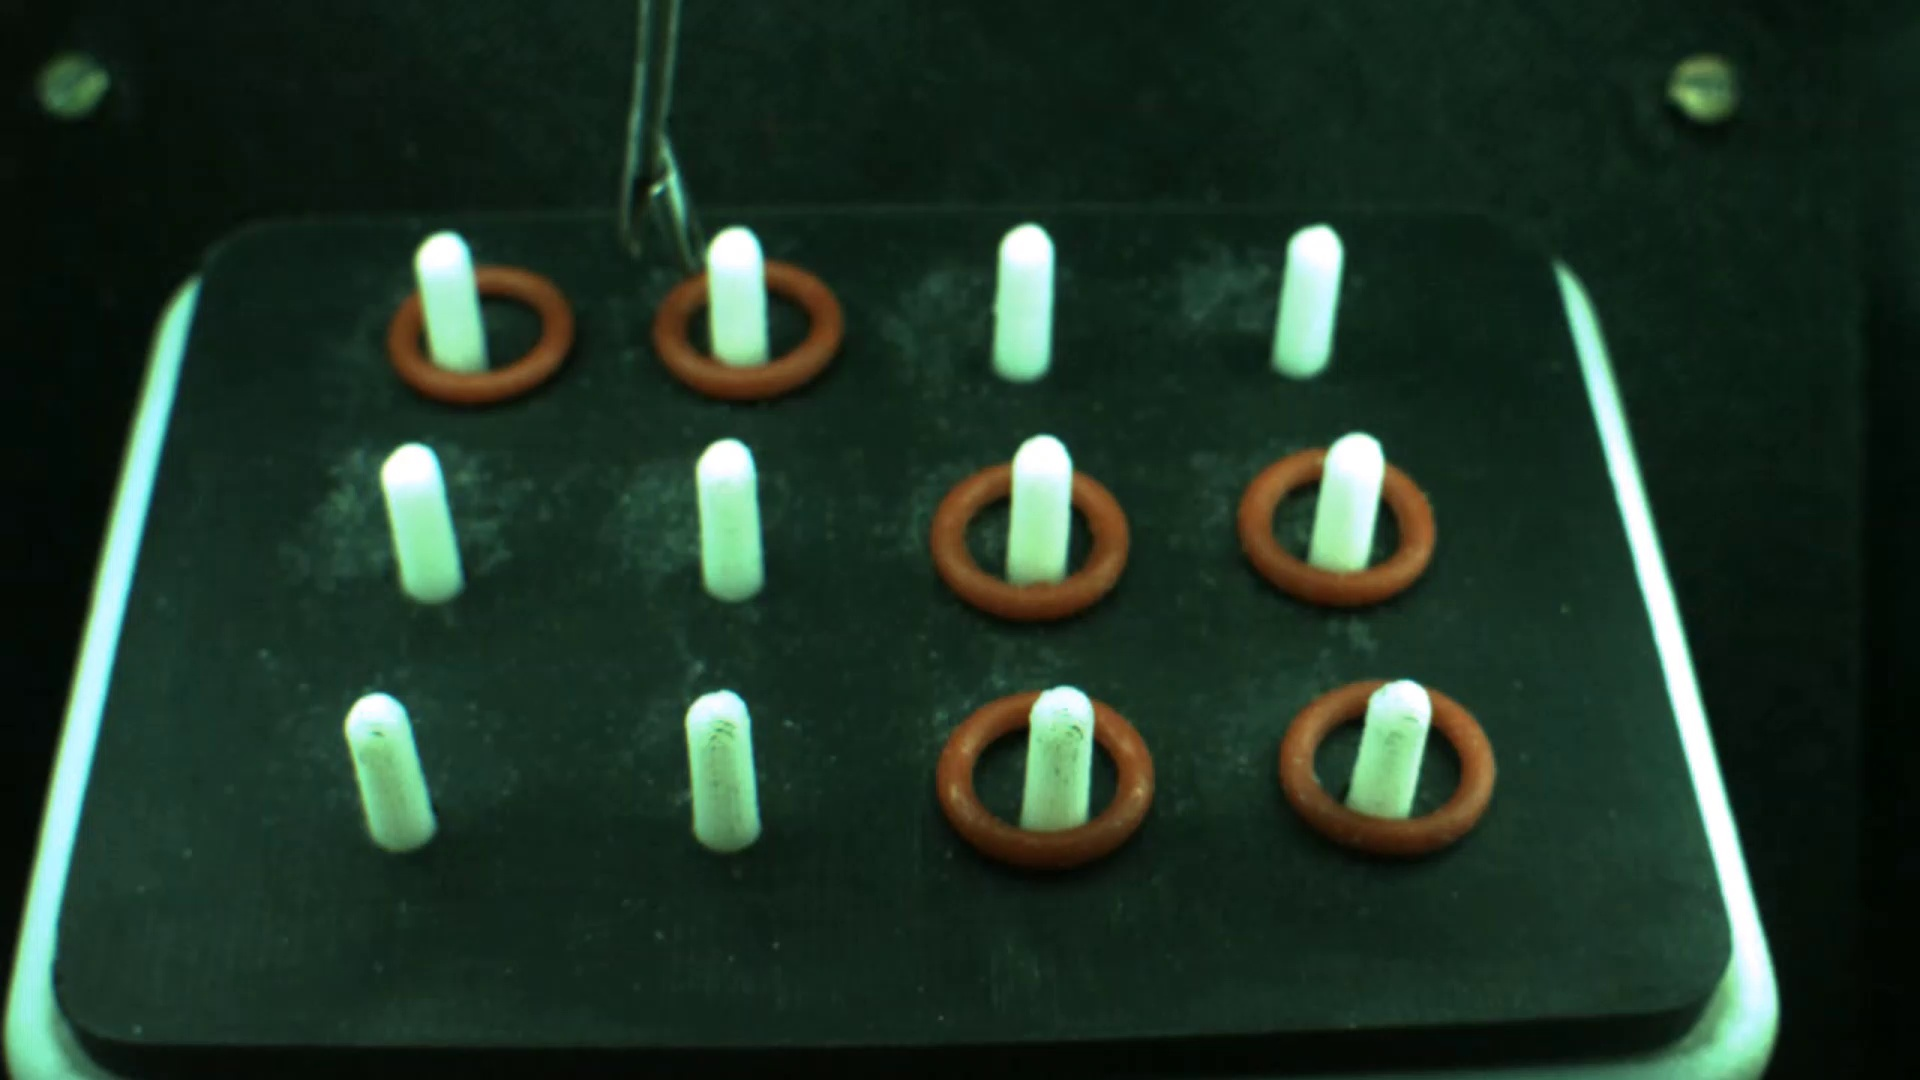
\includegraphics[width=0.23\textwidth]{output/frames/sample3_orig.jpg} &

\includegraphics[width=0.23\textwidth]{output/frames/sample3_fg.jpg} &

\includegraphics[width=0.23\textwidth]{output/frames/sample3_clean.jpg} &
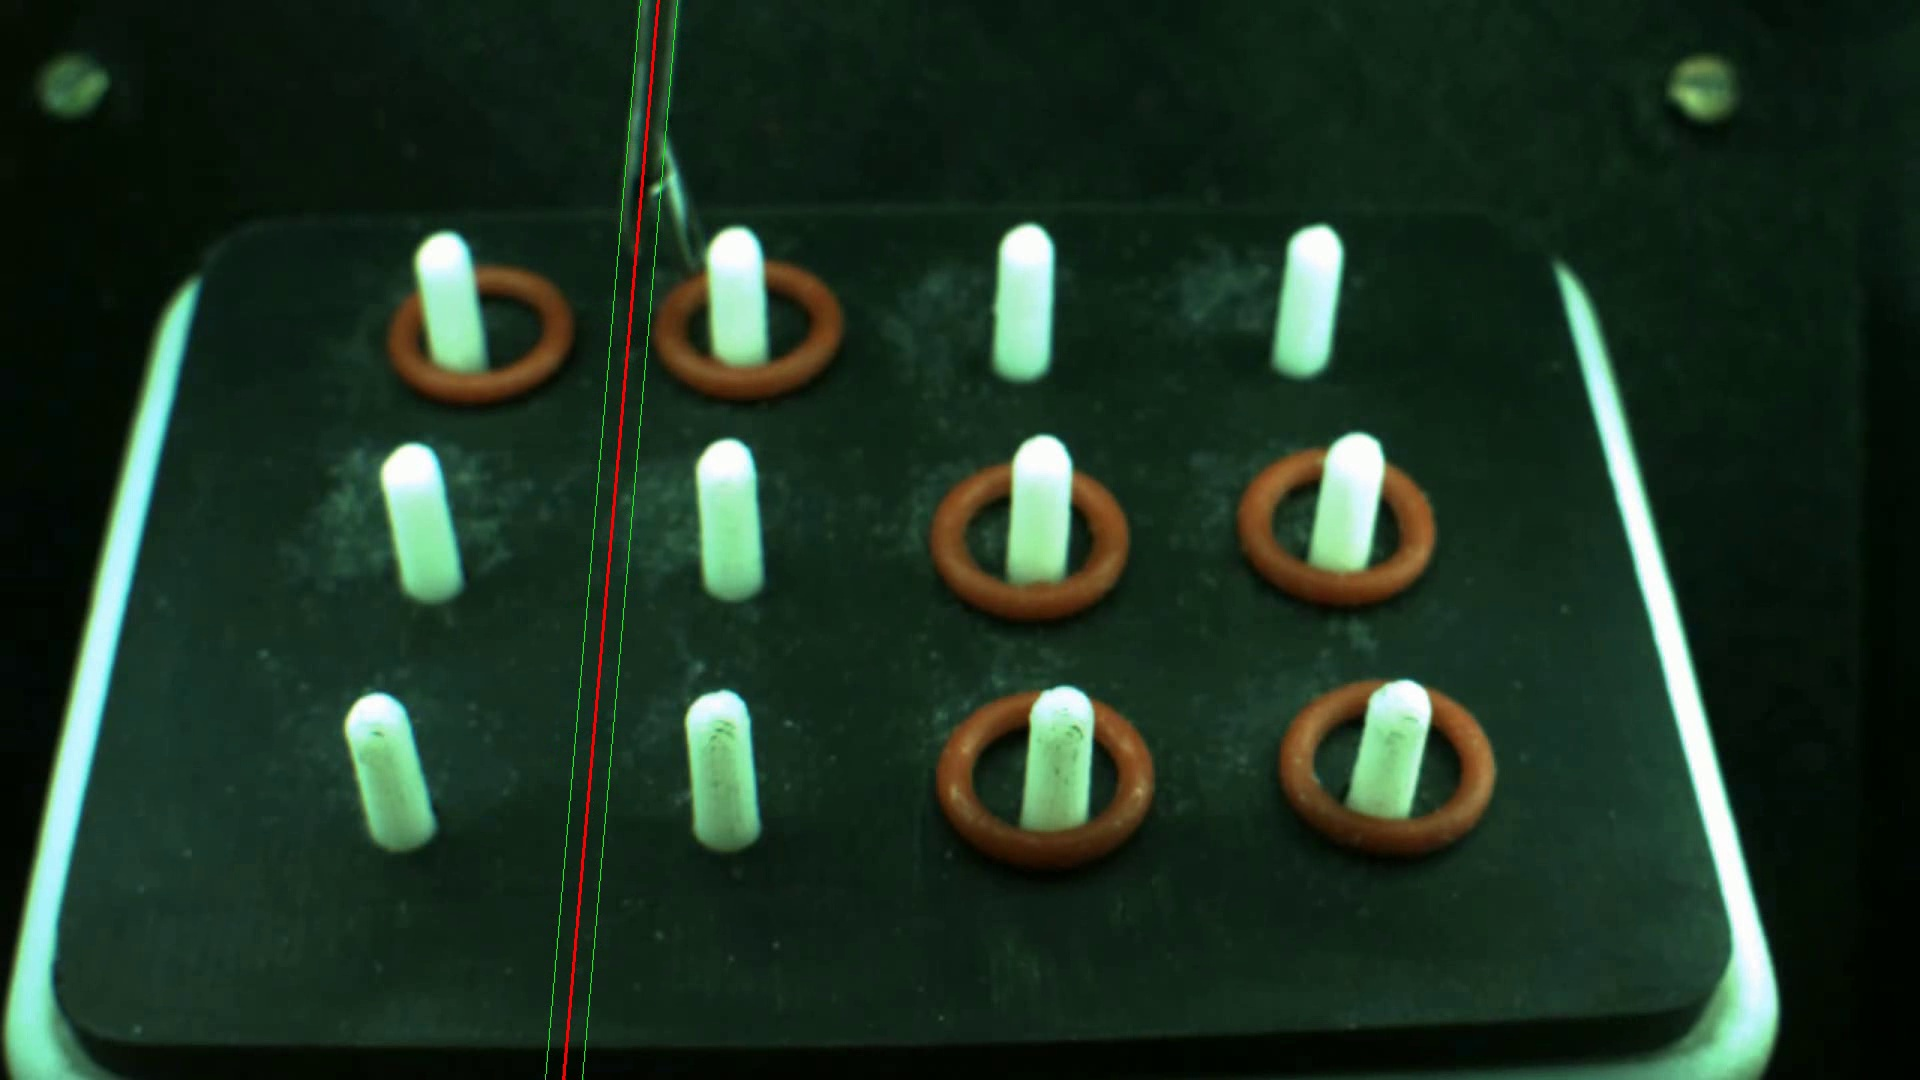
\includegraphics[width=0.23\textwidth]{output/frames/sample3_overlay.jpg} \\
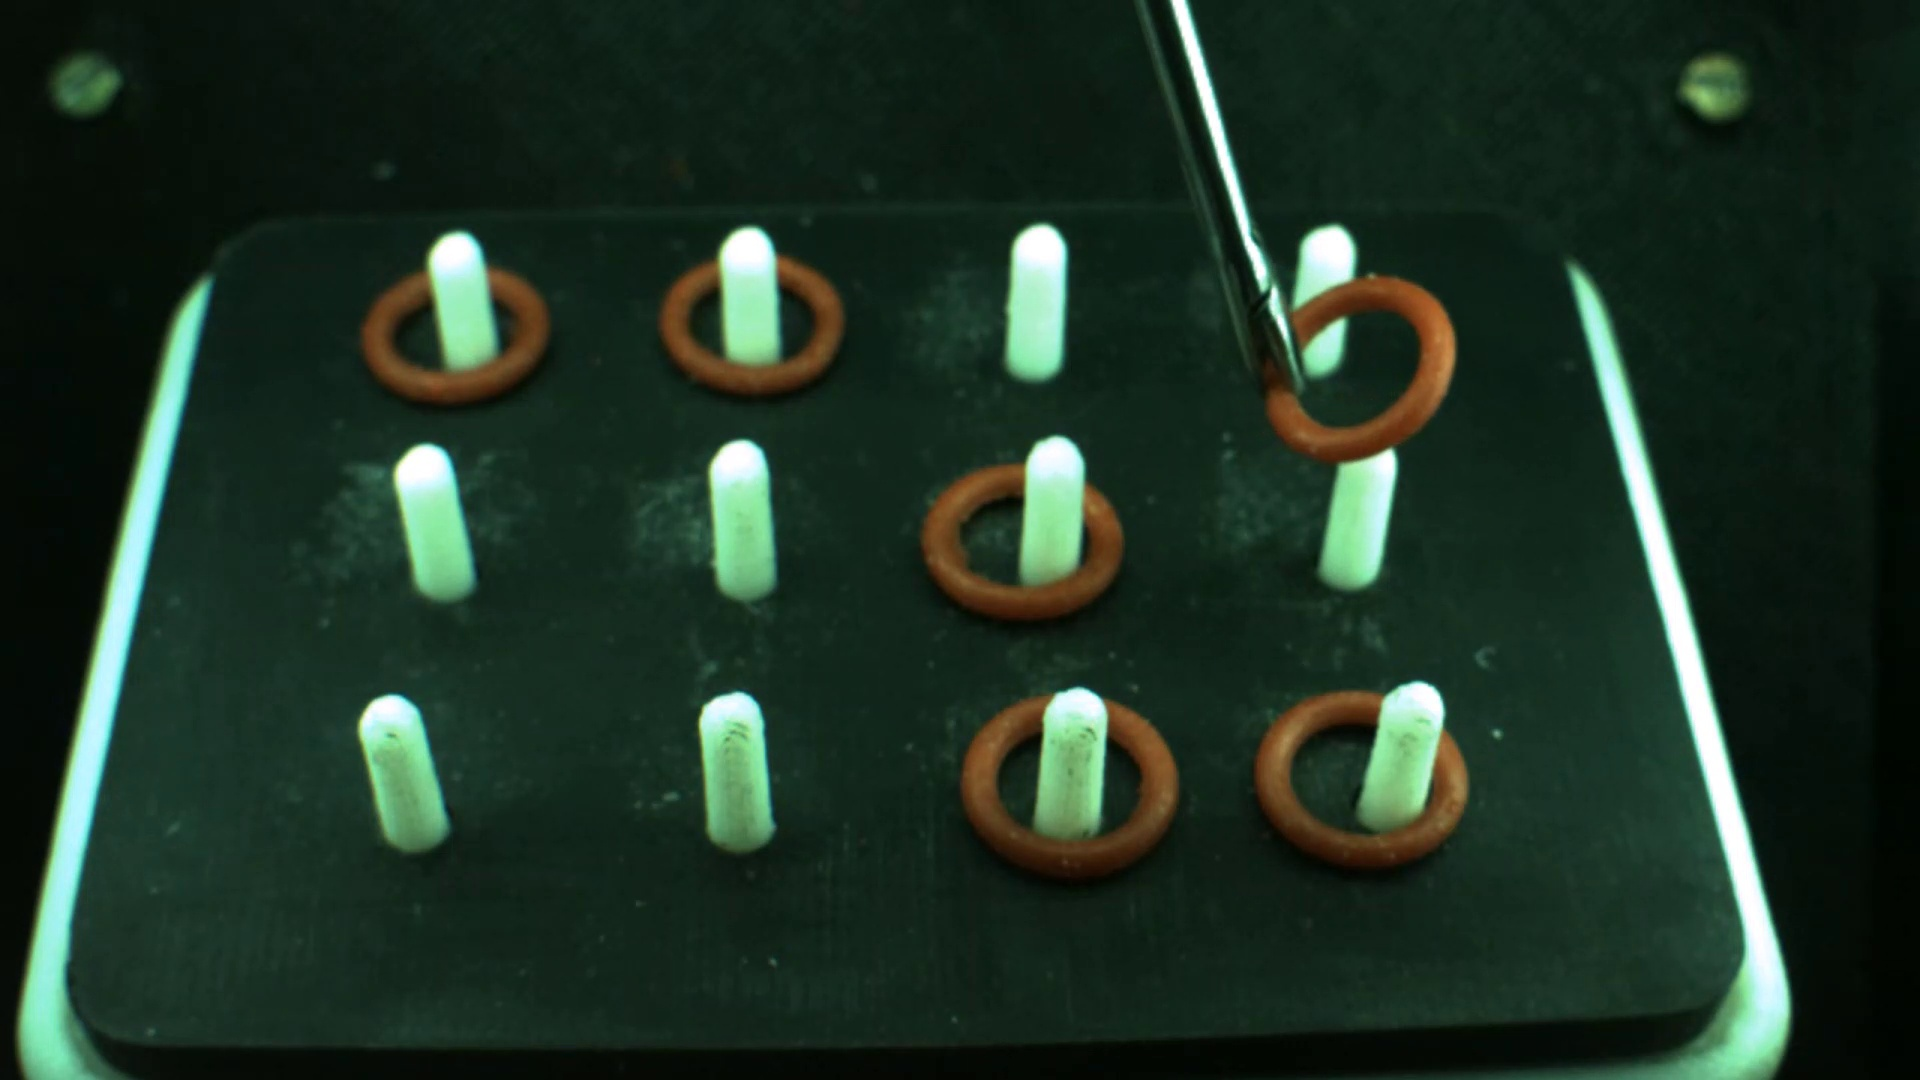
\includegraphics[width=0.23\textwidth]{output/frames/sample4_orig.jpg} &

\includegraphics[width=0.23\textwidth]{output/frames/sample4_fg.jpg} &

\includegraphics[width=0.23\textwidth]{output/frames/sample4_clean.jpg} &
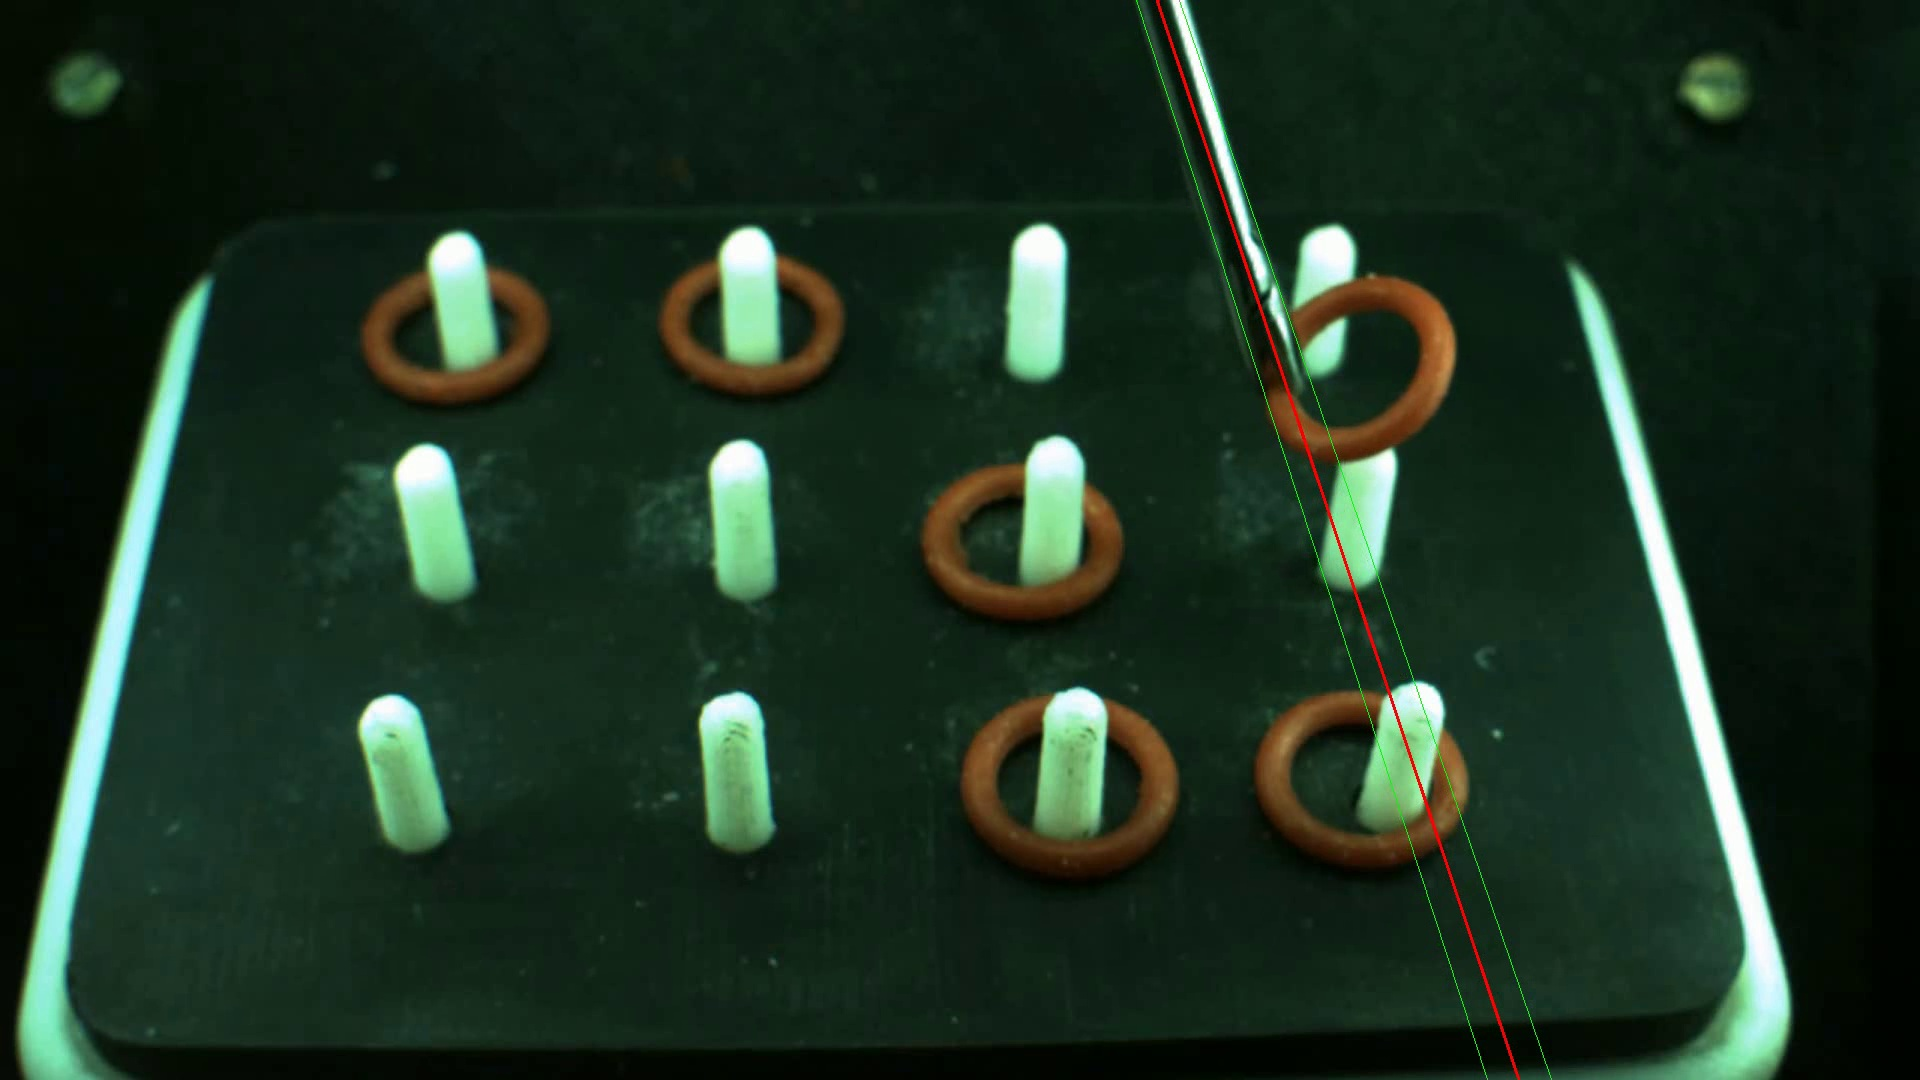
\includegraphics[width=0.23\textwidth]{output/frames/sample4_overlay.jpg} \\
\small Original & \small FG Mask & \small Cleaned & \small Overlay
\end{tabular}
\caption{Pipeline stages for four sample frames across the three input videos. Columns: original frame, foreground mask after background subtraction, morphologically cleaned mask, and final overlay with green edge lines and red medial axis.}
\label{fig:pipeline_stages}
\end{figure*}

% ============================================================================
%  III. RELATED WORK
% ============================================================================
\section{Related Work}

\textbf{Background subtraction} separates foreground (moving objects) from a static background. Methods range from simple frame differencing to statistical models such as MOG, MOG2, and KNN~\cite{opencv}.

\textbf{Hough Line Transform} maps edge points to $(\rho, \theta)$ parameter space via voting. Peaks in the accumulator correspond to dominant lines in image space. It is widely used for line detection in industrial and medical imaging applications~\cite{opencv}.

\textbf{Medial axis / skeleton} is the set of points equidistant from the boundary of an object. For elongated objects such as surgical tools, it reduces to the centreline. It can be computed via morphological thinning or derived from detected boundary lines.

\textbf{Sobel edge detection} is a gradient-based edge detection method using directional derivative kernels to compute image gradients in the $x$ and $y$ directions~\cite{opencv}. The gradient magnitude highlights edge pixels.

% ============================================================================
%  IV. INITIAL ATTEMPTS
% ============================================================================
\section{Initial Attempts}

\subsection{Background Subtraction -- Adaptive Gaussian Mixtures}

The first attempts used adaptive Gaussian Mixture Models, MOG and its extension MOG2~\cite{opencv}, to separate the moving surgical tool from the background. MOG models each pixel's intensity as a mixture of $K$ Gaussians updated online, while MOG2 adds automatic per-pixel selection of the number of components and built-in shadow detection.

Because the videos have a completely static background and can be processed offline (not in real-time), adaptivity offers no benefit: the background never changes, so an adaptive model simply introduces unnecessary complexity. The per-pixel median (used in the final approach) produces the same or better foreground segmentation with a single pass over the video, is computationally cheaper, and yields a deterministic, noise-free background image.

\subsection{Image Processing -- Morphological Experiments}

Various morphological operations were tested during initial attempts, including opening (erosion followed by dilation), combinations of opening and closing with different kernel sizes and shapes (elliptical, rectangular), and additional dilation passes to solidify the tool boundary. In all cases, applying opening deteriorated the output quality: it eroded the thin edges of the surgical tool, causing the Hough Transform to miss edge lines or detect them at incorrect positions. Only morphological closing (used in the final approach) proved beneficial, as it fills interior holes without removing boundary pixels.

\subsection{Medial Axis -- Iterative Refinement}

Three successive approaches were tried for computing the medial axis from a set of detected Hough lines.

\subsubsection{Attempt 1 -- $\rho$/$\theta$ Average with Max-Separation Pairing}

Edge lines were grouped by orientation: lines whose $\theta$ values fell within a tolerance (e.g.\ $\pm 5^\circ$) of the dominant $\theta$ were considered parallel. Among these, the pair with the \emph{largest $\rho$ separation} was selected as the two tool edges, and the medial axis was computed as the arithmetic average of the pair's parameters:
\begin{equation}
    \rho_{\text{med}} = \frac{\rho_1 + \rho_2}{2}, \quad \theta_{\text{med}} = \frac{\theta_1 + \theta_2}{2}
\end{equation}
This works well when the two edges are nearly perfectly parallel, but the simple average drifts when the lines converge slightly, a common occurrence due to perspective and noise.

\subsubsection{Attempt 2 -- Angular Bisector with Same Pairing}

The same max-separation-at-similar-$\theta$ pairing criterion was retained, but the medial axis formula was replaced with a proper angular bisector:
\begin{enumerate}
    \item Compute the intersection point $(x_0, y_0)$ of the two lines.
    \item Obtain unit direction vectors $\hat{d}_1$, $\hat{d}_2$ along each line, aligned so $\hat{d}_1 \cdot \hat{d}_2 > 0$.
    \item The bisector direction is $\hat{b} = (\hat{d}_1 + \hat{d}_2) / \|\hat{d}_1 + \hat{d}_2\|$.
    \item The bisector normal $\hat{n} = (b_y,\, -b_x)^\top$ gives the medial axis parameters:
\end{enumerate}
\begin{equation}
    \theta_b = \arctan2(n_y,\, n_x), \qquad \rho_b = x_0\, n_x + y_0\, n_y
\end{equation}
This improved the medial axis accuracy for non-parallel edges, but the pairing criterion itself was still fragile: picking the two most-separated parallel lines often selected spurious detections rather than the true tool edges.

\subsubsection{Attempt 3 -- Intersection-Filtered Pairing (Final)}

The breakthrough was replacing the pairing criterion. Instead of clustering by $\theta$ alone, all pairs of detected lines are tested geometrically (Section~V, Step~5). This reliably identifies the true tool edges, making the angular bisector formula accurate in practice.

% ============================================================================
%  V. FINAL APPROACH
% ============================================================================
\section{Final Approach}

The final pipeline uses a static per-pixel median background model, morphological closing, Sobel edge detection, a fully vectorised custom Hough Transform, geometrically robust edge-pair selection, and an angular-bisector medial axis computation.

\subsection{Step 1 -- Background Subtraction (Per-pixel Median)}

A static background model is built once by computing the per-pixel median across every frame of the video:
\begin{equation}
    B(x,y) = \underset{t}{\text{median}}\; I_t(x,y)
\end{equation}
For each subsequent frame, the absolute difference is thresholded to obtain a binary foreground mask:
\begin{equation}
    M(x,y) = \bigl[\|I(x,y) - B(x,y)\| > \tau\bigr], \quad \tau = 30
\end{equation}

\textbf{Advantages:} The background in these videos is completely static, so a single median image captures it exactly. Compared to adaptive models (MOG/MOG2), this is computationally simpler (a single pass over all frames, no per-pixel Gaussian updates) and produces a clean, deterministic background with no warm-up artefacts. \textbf{Limitation:} Requires loading all frames into memory once, and cannot adapt to gradual background drift.

\subsection{Step 2 -- Morphological Cleaning}

Only morphological \emph{closing} is applied (dilation followed by erosion), which fills holes in the tool silhouette without eroding the outer boundary:
\begin{lstlisting}
kernel = cv2.getStructuringElement(
             cv2.MORPH_RECT, (9, 9))
cleaned = cv2.morphologyEx(
    fg_mask, cv2.MORPH_CLOSE, kernel,
    iterations=3)
\end{lstlisting}
Opening (which would remove small blobs) was found to erode thin tool edges and was therefore omitted.

\subsection{Step 3 -- Edge Detection (Sobel)}

A Gaussian blur is applied before Sobel derivatives to reduce noise. The gradient magnitude is normalised and thresholded:
\begin{equation}
    |\nabla I| = \sqrt{\left(\frac{\partial I}{\partial x}\right)^2 + \left(\frac{\partial I}{\partial y}\right)^2}
\end{equation}

\subsection{Step 4 -- Custom Hough Line Transform}

\textbf{Accumulator setup:}
\begin{itemize}
    \item $\theta \in [0^\circ, 180^\circ)$, resolution $1^\circ$ ($\to$ 180 bins)
    \item $\rho \in [-d,\, d]$ where $d = \lceil\sqrt{h^2+w^2}\rceil$, resolution $1$\,px
\end{itemize}

\textbf{Voting:} For every edge pixel $(x, y)$, the accumulator is incremented at $\rho = x\cos\theta + y\sin\theta$ for all $\theta$ bins. The voting is fully vectorised using NumPy broadcasting.

\textbf{Peak finding with NMS:} Top peaks are extracted iteratively: the strongest bin is recorded, its neighbourhood ($|\Delta\rho| < 10$\,px, $|\Delta\theta| < 10^\circ$) is zeroed, and the process repeats until the threshold or line count limit is reached.

\subsection{Step 5 -- Edge Pair Selection}

Rather than simply clustering by $\theta$, a geometrically motivated filtering step is applied:

\begin{enumerate}
    \item For every pair of detected lines, compute their intersection point.
    \item \textbf{Discard} pairs whose intersection falls \emph{inside} the image. True tool edges are nearly parallel and must converge outside the frame.
    \item Among surviving pairs, rank by \emph{smallest angular difference} $|\Delta\theta|$ (most parallel first).
    \item Break ties (within $2^\circ$) by \emph{largest spatial separation} measured at the image centre.
    \item If all pairs are eliminated in step~2, fall back to step~4 using all lines.
\end{enumerate}

\subsection{Step 6 -- Medial Axis (Angular Bisector)}

The medial axis is computed using the angular bisector formula described in Section~IV (Attempt~2). When the two selected lines are nearly parallel ($|\Delta\theta| < 10^\circ$), their $\rho$ values are sign-aligned and averaged. When they diverge, the full geometric bisector through the intersection point is used (Eq.~3). This is exact for both parallel and converging edge lines.

\subsection{Step 7 -- Staged Pipeline with Caching}

The pipeline is divided into four stages, each writing its output to disk. On subsequent runs, a stage is skipped if its output file already exists, allowing incremental debugging without reprocessing:
\begin{itemize}
    \item Stage 1: foreground mask video
    \item Stage 2: cleaned mask video
    \item Stage 3: edge map video
    \item Stage 4: medial-axis overlay video + per-frame mode labels
\end{itemize}

\subsection{Step 8 -- Visualization}

Lines are rendered from $(\rho, \theta)$ using:
\begin{equation}
    x = \rho\cos\theta - t\sin\theta, \quad y = \rho\sin\theta + t\cos\theta
\end{equation}
where $t$ ranges across twice the image diagonal. \textbf{Green} lines denote detected edges; the \textbf{red} line denotes the medial axis.

% ============================================================================
%  VI. RESULTS AND OBSERVATION
% ============================================================================
\section{Results and Observation}

Table~\ref{tab:comparison} compares the initial and final approaches.

\begin{table}[H]
\centering
\caption{Initial attempts vs.\ final approach.}
\label{tab:comparison}
\begin{tabular}{@{}lcc@{}}
\toprule
\textbf{Aspect} & \textbf{Initial} & \textbf{Final} \\
\midrule
Background Model  & Adaptive (GMM)     & Static (median)         \\
Complexity        & Higher (online GMM)& Lower (one-pass median) \\
Edge Pairing      & $\theta$-cluster   & Intersection filter     \\
Medial Axis       & $\rho$ average     & Angular bisector        \\
Accuracy          & Moderate           & Improved                \\
\bottomrule
\end{tabular}
\end{table}

The median-based final approach produces a completely clean, static background image in a single pass, computationally cheaper and simpler than the online GMM updates used in initial attempts. Since the background is truly static in these videos, the adaptive models added unnecessary complexity without benefit.

The intersection-filtered edge-pair selection reliably rejects spurious line pairs, and the angular bisector formula for the medial axis is geometrically more accurate than the simple $\rho$ average, especially when the two detected edge lines converge slightly due to perspective or noisy detections.

The pipeline's per-frame mode debug output showed that the majority of frames used the normal intersection-filtered path; the fallback path activated mainly during rapid tool motion or partial occlusion.

% ============================================================================
%  VII. FUTURE WORK
% ============================================================================
\section{Future Work}

\begin{itemize}
    \item \textbf{Out-of-frame handling}: When the tool moves entirely or mostly out of the frame, the pipeline should suppress all line overlays rather than drawing spurious detections on the remaining noise.
    \item \textbf{Circular ring removal}: The tool's circular ring (near the pivot/hinge) is currently picked up during segmentation and can generate false edge lines. A targeted masking or shape-filtering step should be added during image processing to exclude it.
    \item \textbf{Mathematically rigorous edge-pair selection}: The current intersection-filtering criterion works well empirically but is heuristic. A more principled geometric or statistical formulation for selecting the true tool-edge pair from a set of Hough lines would make the pipeline more robust.
    \item \textbf{Adaptive line-detection thresholds}: The Hough vote threshold and NMS radii are currently fixed constants. Adding adaptive thresholds that respond to the number of edge pixels or accumulator statistics per frame would improve robustness across varying tool sizes and motions.
    \item \textbf{Temporal smoothing}: Apply Kalman filtering or exponential moving average to the medial axis parameters $(\rho, \theta)$ across frames for smoother tracking.
    \item \textbf{Multi-tool tracking}: Extend the pipeline to detect and track multiple tools simultaneously by clustering Hough peaks into separate tool groups.
    \item \textbf{Deep learning segmentation}: Replace the background subtraction and edge detection pipeline with a trained segmentation model (U-Net, Mask~R-CNN) for more robust tool detection.
\end{itemize}

% ============================================================================
%  CONCLUSION
% ============================================================================
\section*{Conclusion}

A complete pipeline for medial axis detection of moving surgical tools was developed and refined through iterative experimentation. Early attempts using adaptive Gaussian mixture background subtraction and simple $\theta$-clustering for edge pairing were progressively replaced by a per-pixel median background model (simpler and better suited to the static background), intersection-filtered edge-pair selection, and a geometric angular-bisector medial axis computation. The resulting pipeline produces stable, annotated output videos with green edge overlays and a red medial axis, demonstrating its viability for surgical tool tracking in aerial robotics and computer-assisted intervention systems.

\textit{Acknowledgement:} Rudraksh Gupta supported during the development and debugging of this project.

% ============================================================================
%  REFERENCES
% ============================================================================
\begin{thebibliography}{9}

\bibitem{opencv}
OpenCV, ``OpenCV Documentation,'' \url{https://docs.opencv.org/}, accessed 2025.

\end{thebibliography}

\end{document}
